\documentclass{article}

\usepackage{graphicx}
\usepackage[backend=bibtex]{biblatex}
\usepackage{hyperref} % For clickable URLs

% Bibliography file
\addbibresource{references.bib}

% Title
\title{Prediction of Car Fuel Consumption}
\author{S. Boisgérault}
\date{\today}

\begin{document}

\maketitle

\begin{abstract}
We produce a model that predicts a vehicle fuel consumption from its weight, 
with a estimated standard deviation smaller than 2 liters per 100 km. 
The model is based on the Auto-MPG dataset.
\end{abstract}

\section{Introduction}
\textbf{TODO}

\section{Model}

Our model is:
$$
\mbox{fuel consumption} =  0.00899249 \times \mbox{vehicle weight} -0.90305387
$$
where the fuel consumption is measured in liters per 100 km and the vehicle 
weight in kg.


\begin{figure}[htbp]
    \centering
    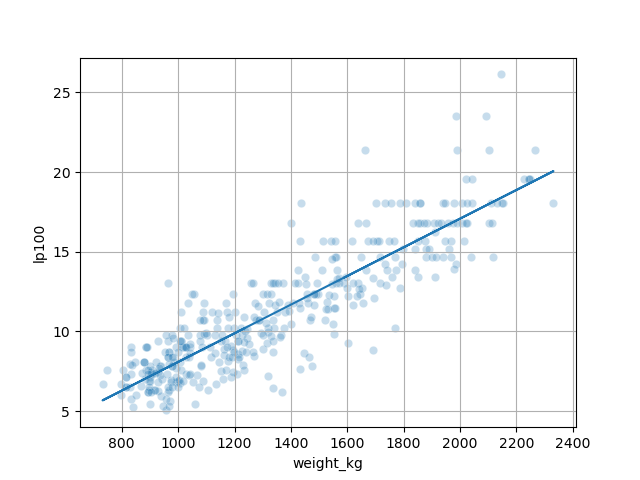
\includegraphics[width=\textwidth]{images/prediction.png} % Replace with your image filename
    \caption{Fuel consumption vs weight in the auto-mpg data sets (semi-transparent dots) 
     and the corresponding prediction model (line).}
    \label{fig:example}
\end{figure}


\section{Error Distribution}

Our model is practically unbiased 
$$
|\mbox{mean}| \leq 10^{-14}
$$
and its standard deviation is
$$
\mbox{std} \approx 1.815 < 2.0.
$$

\begin{figure}[htbp]
    \centering
    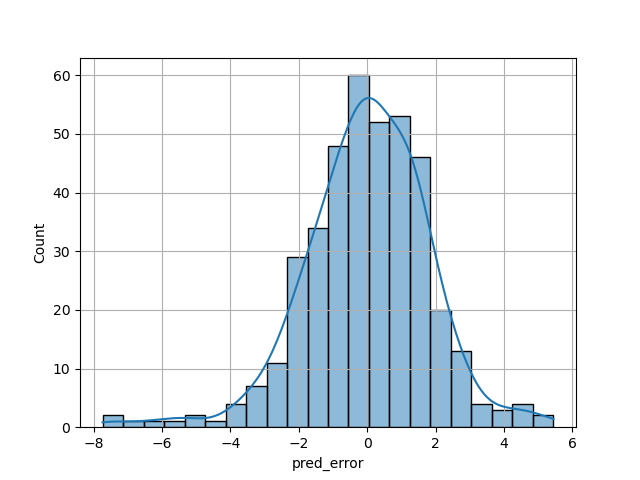
\includegraphics[width=\textwidth]{images/error.png}
    \caption{The consumption prediction error distribution.}
\end{figure}

\section{Dataset}

Auto-mpg comes from \cite{auto_mpg_9}.

\printbibliography

\end{document}
